\clearpage
\section{Opgave 3 - Alarm Watch}
\begin{enumerate}
	\item[1)]
	Vi lægger yderligere en vhdl-fil ovenpå, og bruger structural style til at bygge vores elementer ud af de tidligere programmerede enheder "watch", "counter" og "bcd-decoder". 
	
	Vi ændrer dog i bin-value fra de underlæggende filer, således at vi kan sammenligne signal-værdier mellem klokkens værdi, og den alarmtid som vi sætter. 
	
	Når alarmen udløses, lader vi LEDR0 lyse rødt, som det fremgår på billederne under koden.

	VHDL-koden for programmet er følgende:
	
	\begin{lstlisting}[caption={Koden for øverste lag af Alarm Watch},label={lst:alarmWatch}]
		
	library ieee;
use ieee.std_logic_1164.all;
use ieee.numeric_std.all;

entity Alarm is
port (clk, reset, view, speed: in std_logic;
		AL_MIN_1, AL_MIN_10, AL_HOUR_1, AL_HOUR_10: in std_logic_vector(3 downto 0);
		seg1, seg10, seg100, seg1000, seg10000, seg100000: out std_logic_vector(6 downto 0);
		ALARM : out std_logic);
		end Alarm;
		
architecture TimingAlarm of Alarm is

signal AL_MIN_1_SIG, AL_MIN_10_SIG,AL_HOUR_1_SIG, AL_HOUR_10_SIG : std_logic_vector(3 downto 0);
signal comp_min1, comp_min10, comp_hour1, comp_hour10 : std_logic_vector (3 downto 0);
signal a_seg1, a_seg10, a_seg100, a_seg1000, a_seg10000, a_seg100000 : std_logic_vector(6 downto 0);
signal i_seg1, i_seg10, i_seg100, i_seg1000, i_seg10000, i_seg100000 : std_logic_vector(6 downto 0);
signal seg1_sig, seg10_sig, seg100_sig, seg1000_sig, seg10000_sig, seg100000_sig : std_logic_vector(6 downto 0);

begin

VisAlarm1: entity work.BCDdecoder port map(dcba=>"0000", seg => a_seg1);
VisAlarm10: entity work.BCDdecoder port map(dcba=>"0000", seg => a_seg10);
VisAlarm100: entity work.BCDdecoder port map(dcba=>AL_MIN_1_SIG, seg => a_seg100);
VisAlarm1000: entity work.BCDdecoder port map(dcba=>AL_MIN_10_SIG, seg => a_seg1000);
VisAlarm10000: entity work.BCDdecoder port map(dcba=>AL_HOUR_1_SIG, seg => a_seg10000);
VisAlarm100000: entity work.BCDdecoder port map(dcba=>AL_HOUR_10_SIG, seg => a_seg100000);

VisUr: entity work.watch_ext port map(
	seg1 => i_seg1, 
	seg10 => i_seg10, 
	seg100 => i_seg100, 
	seg1000 => i_seg1000, 
	seg10000 => i_seg10000, 
	seg100000 => i_seg100000,
	bin_val_m1 => comp_min1,
	bin_val_m10 => comp_min10,
	bin_val_h1 => comp_hour1,
	bin_val_h10 => comp_hour10,
	speed => speed,
	clk=>clk,
	reset=>reset);

process (view)
begin 

	if AL_MIN_1 >= "1001" then
		AL_MIN_1_SIG<="1001";
	else 
		AL_MIN_1_SIG<=AL_MIN_1;
	end if;
	
	if AL_MIN_10 >= "0101" then
		AL_MIN_10_SIG <= "0101";
	else 
		AL_MIN_10_SIG<=AL_MIN_10;
	end if;
	
	if AL_HOUR_1 >= "1001" and AL_HOUR_10 <="0001" then
		AL_HOUR_1_SIG <= "1001";
	elsif AL_HOUR_1>="0011" and AL_HOUR_10 >="0010" then
		AL_HOUR_1_SIG <= "0011";
	else
		AL_HOUR_1_SIG <= AL_HOUR_1;
	end if;
	
	if AL_HOUR_10 >= "0010" then
		AL_HOUR_10_SIG <= "0010";
	else
		AL_HOUR_10_SIG <= AL_HOUR_10;
	end if;
	
	if view ='0' then
		Seg1<=i_seg1;
		Seg10<=i_seg10;
		Seg100 <=i_seg100;
		Seg1000 <= i_seg1000;
		Seg10000<= i_seg10000;
		Seg100000<= i_seg100000;
	
	elsif view ='1' then
		Seg1<=a_seg1;
		Seg10<=a_seg10;
		Seg100 <= a_seg100 ;
		Seg1000 <= a_seg1000;
		Seg10000<= a_seg10000;
		Seg100000<= a_seg100000;
	end if;
	
	if AL_MIN_1_SIG & AL_MIN_10_SIG & AL_HOUR_1_SIG & AL_HOUR_10_SIG = comp_min1 & comp_min10 & comp_hour1 & comp_hour10 then
		ALARM <= '1';
	else
		ALARM <= '0';
	end if;
	
end process;

end TimingAlarm;

\end{lstlisting}


\begin{figure}[h]
	\centering
	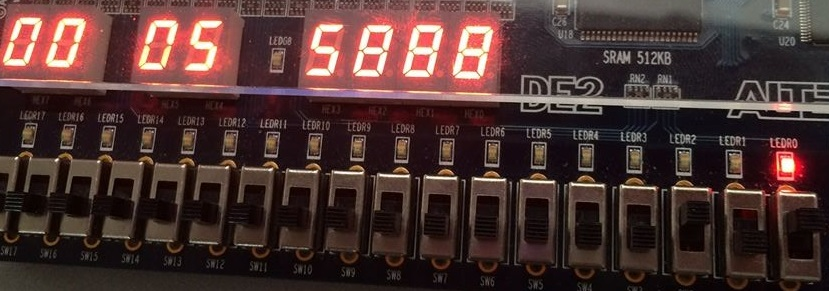
\includegraphics[scale=0.45]{pictures/Oevelse6/opg3/AlarmOn.JPG}
	\caption{Alarm er igang (LEDR0 lyser)}
	\label{fig:alarmOn}
\end{figure}

\begin{figure}[h]
	\centering
	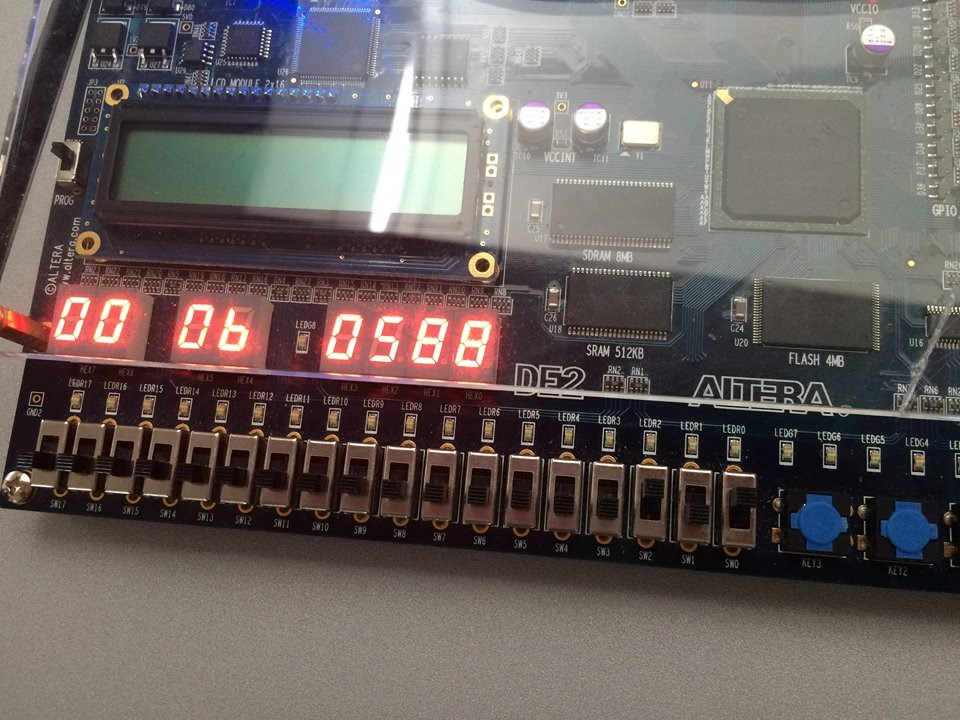
\includegraphics[scale=0.45]{pictures/Oevelse6/opg3/AlarmOff.JPG}
	\caption{Alarm er ikke aktiv (LEDR0 lyser ikke)}
	\label{fig:alarmOff}
\end{figure}

\begin{figure}[h]
	\centering
	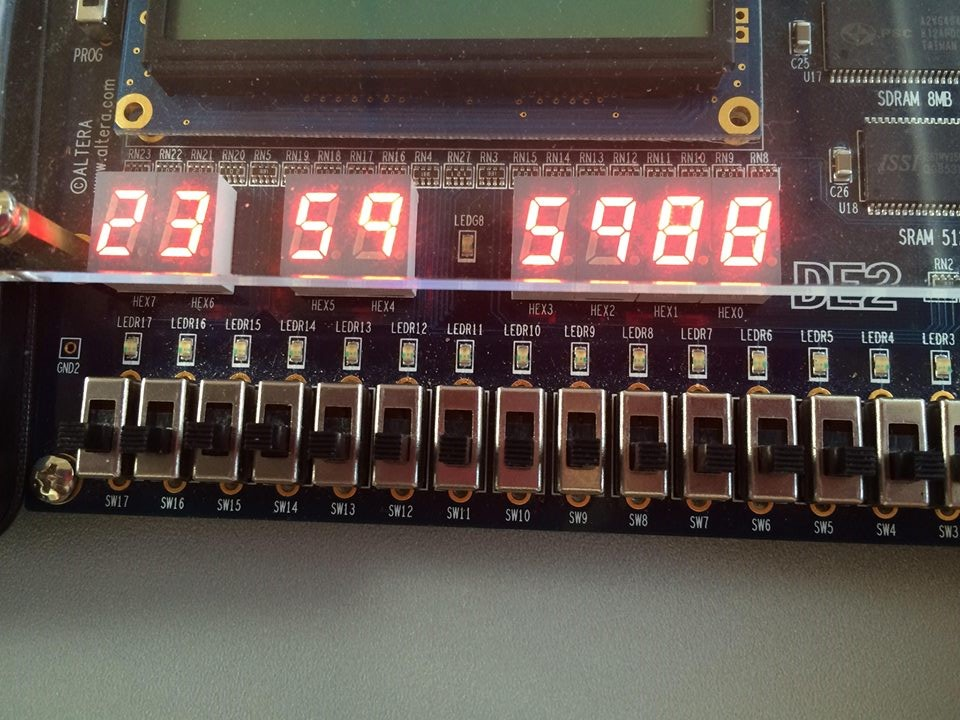
\includegraphics[scale=0.45]{pictures/Oevelse6/opg3/AlarmMaxValue.JPG}
	\caption{Alarm har nået maksimal værdi}
	\label{fig:alarmMaxValue}
\end{figure}


\end{enumerate}
	